
\chapter{準備}
\label{chap:preliminary}
本章では,後の章に向けての準備をする.はじめに,グラフ理論の基本事項を説明する.
頂点間距離や直径などを含む.次に,Cerfらが提案した一般化ムーアグラフの
定義を与え,いくつかの性質を示す.これらの性質は,一般化ムーアグラフを
探索する方法に用いるもので,極めて重要である.

\section{グラフ理論の基本事項}
\label{sect:basic-graph-theory}
グラフ理論の基本事項を,\cite{Diestel2000}の記号に則り説明する.
グラフ理論の基礎を理解している読者は\ref{sect:generalized-moore-graph}節まで
読み飛ばしても差し支えない.

\textbf{グラフ}とは,二つの集合$V$と$E$の組$G=(V,E)$で,$E$は
$E\subseteq[V]^2$つまり,$V$から重複なく元を2個取り出した集合の部分集合である.
$V$を\textbf{頂点集合}とよび,その元を\textbf{頂点}とよぶ.
また,頂点集合の大きさ$|V|$を\textbf{頂点数}とよぶ.
$E$を\textbf{辺集合}とよび,その元を\textbf{辺}とよぶ.
後で示すように,グラフを図示する際,頂点は丸や点で,辺は頂点を結ぶ線で
表されることが多い.

頂点$v$と辺$e$が\textbf{接続する}とは,$v\in e$つまり,$e$の端点に$v$が
属することをいう.頂点$v$と頂点$w$が\textbf{隣接する}とは,$\{v,w\}$が
辺集合に属することをいう.

グラフ$G$上の頂点$v$に対して,その頂点と隣接している頂点の数を
\textbf{次数}と呼び,$d_G(v)$あるいは$d(v)$と記す.
すべての頂点について,その次数が一定のグラフを\textbf{正則グラフ}と呼ぶ.

\textbf{経路}$P$とは,$P=(V,E)$のグラフで,
\[ V=\{x_0,x_1,\ldots,x_k\},\:
E=\{\{x_0,x_1\},\{x_1,x_2\},\ldots,\{x_{k-1},x_k\}\}\]
を満たす$V$と$E$の組である.このときの辺の数を経路の\textbf{長さ}あるいは
\textbf{経路長}という.長さが2以上の閉路$P$に対して,その両端の頂点を
隣接させたグラフを\textbf{閉路}という.つまり,閉路$C=(V,E)$とは,
\[ V=\{x_0,x_1,\ldots,x_{k-1}\},\:
E=\{\{x_0,x_1\},\{x_1,x_2\},\ldots,\{x_{k-2},x_{k-1}\},\{x_{k-1},x_0\}\}\]
を満たす,$k\geq0$のグラフである.閉路$C$の辺の数あるいは頂点の数を,
閉路の\textbf{長さ}あるいは\textbf{閉路長}とよぶ.

グラフ$G$上の頂点$v$と$w$について,$v$と$w$を結ぶ最短の経路の長さを$v$と$w$の
\textbf{頂点間距離}とよび,$d_G(v,w)$あるいは$d(v,w)$で表す.
$v$と$w$を結ぶ経路が存在しないとき,$d(v,w):=\infty$と定義する.
経路の対称性より,$d(v,w)=d(w,v)$である.すべての二頂点の組合せに対する
頂点間距離の平均値と最大値をそれぞれ\textbf{平均頂点間距離}と\textbf{直径}
という.

\begin{example}
  図\ref{fig:graph-example}にグラフの例を示す.
  頂点集合は
  $\{u,v,w,x,y,z\}$
  で,辺集合は
  $\{(u,w),(v,x),(w,x),(w,y),(x,z),(y,z)\}$
  である.次数は,それぞれの頂点に対して,
  $d(u)=1,\,d(v)=1,\,d(w)=3,\,d(x)=3,\,d(y)=2,\,d(z)=2$
  である.グラフには,長さ4の閉路
  $\{w,x,z,y\}$
  が存在する.頂点間距離は次のとおり.
  \begin{equation*}
    \begin{aligned}
      d(u,v)=3&\:&d(u,w)=1&\:&d(u,x)=2&\:&d(u,y)=2&\:&d(u,z)=3 \\
      &\:&d(v,w)=2&\:&d(v,x)=1&\:&d(v,y)=3&\:&d(v,z)=2 \\
      &\:&&\:&d(w,x)=1&\:&d(w,y)=1&\:&d(w,z)=2 \\
      &\:&&\:&&\:&d(x,y)=2&\:&d(x,z)=1 \\
      &\:&&\:&&\:&&\:&d(y,z)=1 \\
    \end{aligned}
  \end{equation*}
  平均頂点間距離は,頂点間距離の値の平均を求めると,$1.8$である.
  直径は,頂点間距離の値の最大値なので,$3$である.
  \begin{figure}
    \centering
    \input{graph-example.pdf_tex}
    \caption{グラフの例}
    \label{fig:graph-example}
  \end{figure}
\end{example}

\section{一般化ムーアグラフ}
\label{sect:generalized-moore-graph}
本節では一般化ムーアグラフを定義する.
さらに,これが満たすいくつかの性質を示す.

\begin{definition}[Cerf et.al., 1973\,\cite{Cerf1973}]
  \label{def:generalized-moore-graph}
  次の性質が成り立つ頂点数$n$,次数$k$の正則グラフを
  \textbf{一般化ムーアグラフ}(\textbf{Generalized Moore graph})とよぶ.

  すべての頂点$v$について,$v$から$i$離れた頂点の数
  $c_i = \lvert\{ w\,|\,d(v,w) = i , w\in V \}\rvert$について,
  \begin{equation}
    \label{eq:gmg-verts-dist}
    \begin{aligned}
      c_i =
      \begin{cases}
        k(k-1)^{i-1} & 1\leq i\leq Q \\
        R & i = Q+1 \\
        0 & Q+2\leq i \leq n-1
      \end{cases}
    \end{aligned}
  \end{equation}
  であること.ただし,
  \begin{align}
    Q(n,k)&=\max\{q|n-1-\sum_{i=1}^{q}k(k-1)^{i-1}\geq 0\}\label{eq:gmg-q} \\
    R(n,k)&=n-1-\sum_{i=1}^{Q(n,k)}k(k-1)^{i-1}\label{eq:gmg-r}
  \end{align}
  とする.
\end{definition}
\begin{example}
  頂点数12,次数3の一般化ムーアグラフを考える.そのようなグラフを
  \begin{figure}
    \centering
    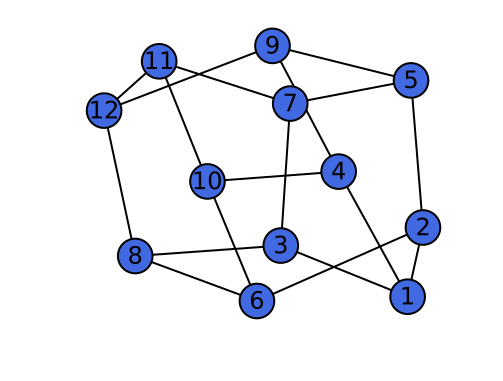
\includegraphics[width=.6\textwidth]{gmg-example-bignode.pdf}
    \caption{頂点数12,次数3の一般化ムーアグラフの例}
    \label{fig:moore-graph-example}
  \end{figure}
  図\ref{fig:moore-graph-example}に示したグラフを考える.
  $Q(12,3)$と$R(12,3)$はそれぞれ,
  \begin{align*}
    Q(12,3) &= \max\{q | 12-1-\sum_{i=1}^{q}3\cdot2^{i-1} \geq 0\} = 2 \\
    R(12,3) &= 12 - 1 - \sum_{i=1}^{Q(12,3)}3\cdot2^{i-1} = 2
  \end{align*}
  である.このグラフの頂点$1$に着目する.頂点$1$からの距離によって,
  残りの頂点を分類する.
  \begin{enumerate}
  \item 頂点$1$からの距離が$1$の頂点は$\{2,3,4\}$
  \item 頂点$1$からの距離が$2$の頂点は$\{5,6,7,8,9,10\}$
  \item 頂点$1$からの距離が$3$の頂点は$\{11,12\}$
  \end{enumerate}
  である.$1$からの距離が$i$の頂点数$c_i$は,
  \begin{align*}
  c_1 &= 3\cdot2^0 = 3 & \\
  c_2 &= 3\cdot2^1 = 6 & \\
  c_3 &= R(12,3) = 2 & \\
  c_i &= 0 & (i>3)
  \end{align*}
  となるので,式\ref{eq:gmg-verts-dist}で示した距離と頂点数の
  関係を満たす.同様に,他のすべての頂点について,上述の距離と頂点数の関係を
  満たす.よって,このグラフは一般化ムーアグラフである.
\end{example}
以下,頂点数$n$,次数$k$の一般化ムーアグラフを$M(n,k)$と記し,
$Q(n,k)$と$R(n,k)$をそれぞれ式\ref{eq:gmg-q}と式\ref{eq:gmg-r}のとおりとする.
頂点数と次数が文脈から明らかな場合は省略してそれぞれ$M,Q,R$と表す.

一般化ムーアグラフの頂点間距離の総和を求め,これが正則グラフの頂点間距離の総和の
下界であることを示す.
\begin{theorem}[Cerf et.al., 1974\,\cite{Cerf1974Lower}]
  \label{thm:gmg-lower-bound}
  $M(n,k)$の頂点間距離の総和は,
  \begin{equation}
    \label{eq:gmg-lb}
    S(n,k) = \sum_{(s,t)\in V\times V}d(s,t) =
    n \left[\ \sum^{Q}_{i=1}ik(k-1)^{i-1} + (Q+1)R\ \right]
  \end{equation}
  で与えられる.これは,正則グラフの頂点間距離の総和の下界である.
\end{theorem}
\begin{proof}
  ある頂点$v$から頂点$w(\neq v)$との距離の総和を次式で表す.
  \begin{equation}
    \label{eq:gmg-lb-1}
    \sum_{i=1}^{n-1}i c_i
  \end{equation}
  ここで,$c_i$は$v$との距離が$i$の頂点の個数とする.
  一般化ムーアグラフの場合,$c_i$は式\ref{eq:gmg-verts-dist}で与えられる.
  そのため,式\ref{eq:gmg-lb-1}から,
  \begin{align}
      \sum_{i=1}^{n-1}ic_i
      &=\sum_{i=1}^{Q}ic_i+(Q+1)c_{Q+1}+\sum_{i=Q+2}^{n-1}ic_i \nonumber\\
      &=\sum_{i=1}^{Q}ik(k-1)^{i-1}+(Q+1)R
      \label{eq:gmg-lb-2}
  \end{align}
  が得られる.これは一つの頂点から他のすべての頂点への距離の総和を表すので,
  式\ref{eq:gmg-lb-2}を$n$倍すると,式\ref{eq:gmg-lb}が得られる.

  次に,式\ref{eq:gmg-lb}が頂点間距離の総和の下界であることを示す.
  一般的な$c'_i$に対して,
  \begin{equation}
    \label{eq:gmg-lb-3}
    \sum_{i=1}^{n-1}i c_i \leq \sum_{i=1}^{n-1}i c'_i
  \end{equation}
  であることを証明する.
  $1\leq i\leq Q$の範囲で,$c_i$は最大なので次が得られる.
  \begin{equation}
    \label{eq:gmg-lb-4}
    \begin{aligned}
      c_i - c'_i
      \begin{cases}
        \geq 0 & 1\leq i\leq Q \\
        \lesseqgtr 0 & i = Q+1 \\
        \leq 0 & Q+2\leq i\leq n-1
      \end{cases}
    \end{aligned}
  \end{equation}
  $c_{Q+1}\geq c'_{Q+1}$と$c_{Q+1}\leq c'_{Q+1}$のふたつの場合について考える.
  \begin{enumerate}[(i)]
  \item $c_{Q+1}\geq c'_{Q+1}$のとき
  \end{enumerate}
  $c_{Q+1}\geq c'_{Q+1}$ならば$c_{Q+1}-c'_{Q+1}\geq0$となり,
  式\ref{eq:gmg-lb-4}より,
  \begin{equation}
    \label{eq:gmg-lb-5a}
    \begin{aligned}
      c_i-c'_i
      \begin{cases}
        \geq 0 & 1\leq i\leq Q+1 \\
        \leq 0 & Q+2\leq i\leq n-1
      \end{cases}
    \end{aligned}
  \end{equation}
  が成り立つ.$c_i$の定義より,次が成り立つ.
  \begin{equation}
    \label{eq:gmg-lb-6}
    \sum_{i=1}^{n-1}c_i = \sum_{i=1}^{n-1}c'_i = n-1
  \end{equation}
  式\ref{eq:gmg-lb-5a}と式\ref{eq:gmg-lb-6}より,
  \begin{equation}
    \label{eq:gmg-lb-7a}
    \begin{aligned}
      \sum_{i=1}^{Q+1}(c_i-c'_i) &= \sum_{i=1}^{Q+1}|c_i-c'_i| \\
      \sum_{i=Q+2}^{n-1}(c_i-c'_i) &= -\sum_{i=Q+2}^{n-1}|c_i-c'_i| \\
      \sum_{i=1}^{Q+1}|c_i-c'_i| &= \sum_{i=Q+2}^{n-1}|c_i-c'_i|
    \end{aligned}
  \end{equation}
  が得られる.式\ref{eq:gmg-lb-7a}を用いて,式\ref{eq:gmg-lb-8a}を考える.
  \begin{equation}
    \label{eq:gmg-lb-8a}
    \sum_{i=1}^{n-1}i(c_i-c'_i)=
    \sum_{i=1}^{Q+1}i|c_i-c'_i|-\sum_{i=Q+2}^{n-1}|c_i-c'_i|
  \end{equation}
  式\ref{eq:gmg-lb-8a}の第一項の上界は,式\ref{eq:gmg-lb-8a1}である.
  \begin{equation}
    \label{eq:gmg-lb-8a1}
    \sum_{i=1}^{Q+1}i|c_i-c'_i|\leq (Q+1)\sum_{i=1}^{Q+1}|c_i-c'_i|
  \end{equation}
  式\ref{eq:gmg-lb-8a}の第二項の下界は,式\ref{eq:gmg-lb-8a2}である.
  \begin{equation}
    \label{eq:gmg-lb-8a2}
    \sum_{i=Q+2}^{n-1}i|c_i-c'_i|\geq (Q+2)\sum_{i=Q+2}^{n-1}|c_i-c'_i|
  \end{equation}
  式\ref{eq:gmg-lb-8a1}と式\ref{eq:gmg-lb-8a2}より,次が成り立つ.
  \begin{align*}
    \sum_{i=1}^{n-1}i(c_i-c'_i)
    &\leq (Q+1)\sum_{i=1}^{Q+1}|c_i-c'_i|-(Q+2)\sum_{i=Q+2}^{n-1}|c_i-c'_i| \\
    &= (Q+1)\sum_{i=1}^{Q+1}|c_i-c'_i|-(Q+2)\sum_{i=1}^{Q+1}|c_i-c'_i| \\
    &= -\sum_{i=1}^{Q+1}|c_i-c'_i| \\
    &\leq 0
  \end{align*}
  ゆえに式\ref{eq:gmg-lb-3}が成り立つ.

  \begin{enumerate}[(i)]
    \setcounter{enumi}{1}
  \item $c_{Q+1}\leq c'_{Q+1}$の場合もほとんど同じである.
  \end{enumerate}
  $c_{Q+1}\leq c'_{Q+1}$ならば$c_{Q+1}-c'_{Q+1}\leq0$となり,
  式\ref{eq:gmg-lb-4}より,
  \begin{equation}
    \label{eq:gmg-lb-5b}
    \begin{aligned}
      c_i-c'_i
      \begin{cases}
        \geq 0 & 1\leq i\leq Q \\
        \leq 0 & Q+1\leq i\leq n-1
      \end{cases}
    \end{aligned}
  \end{equation}
  式\ref{eq:gmg-lb-5b}と式\ref{eq:gmg-lb-6}より,
  \begin{equation}
    \label{eq:gmg-lb-7b}
    \begin{aligned}
      \sum_{i=1}^{Q}(c_i-c'_i) &= \sum_{i=1}^{Q}|c_i-c'_i| \\
      \sum_{i=Q+1}^{n-1}(c_i-c'_i) &= -\sum_{i=Q+1}^{n-1}|c_i-c'_i| \\
      \sum_{i=1}^{Q}|c_i-c'_i| &= \sum_{i=Q+1}^{n-1}|c_i-c'_i|
    \end{aligned}
  \end{equation}
  が得られる.式\ref{eq:gmg-lb-7a}を用いて,次の式\ref{eq:gmg-lb-8b}を考える.
  \begin{equation}
    \label{eq:gmg-lb-8b}
    \sum_{i=1}^{n-1}i(c_i-c'_i)=
    \sum_{i=1}^{Q}i|c_i-c'_i|-\sum_{i=Q+1}^{n-1}|c_i-c'_i|
  \end{equation}
  式\ref{eq:gmg-lb-8b}の第一項の上界は,次の式\ref{eq:gmg-lb-8b1}である.
  \begin{equation}
    \label{eq:gmg-lb-8b1}
    \sum_{i=1}^{Q}i|c_i-c'_i|\leq Q\sum_{i=1}^{Q}|c_i-c'_i|
  \end{equation}
  式\ref{eq:gmg-lb-8b}の第二項の下界は,次の式\ref{eq:gmg-lb-8b2}である.
  \begin{equation}
    \label{eq:gmg-lb-8b2}
    \sum_{i=Q+1}^{n-1}i|c_i-c'_i|\geq (Q+1)\sum_{i=Q+1}^{n-1}|c_i-c'_i|
  \end{equation}
  式\ref{eq:gmg-lb-8b1}と式\ref{eq:gmg-lb-8b2}より,次が成り立つ.
  \begin{align*}
    \sum_{i=1}^{n-1}i(c_i-c'_i)
    &\leq Q\sum_{i=1}^{Q}|c_i-c'_i|-(Q+1)\sum_{i=Q+1}^{n-1}|c_i-c'_i| \\
    &= Q\sum_{i=1}^{Q}|c_i-c'_i|-(Q+1)\sum_{i=1}^{Q}|c_i-c'_i| \\
    &= -\sum_{i=1}^{Q}|c_i-c'_i| \\
    &\leq 0
  \end{align*}
  ゆえに式\ref{eq:gmg-lb-3}が成り立つ.
\end{proof}

\begin{example}
  再び$M(12,3)$について考える.$M(12,3)$の頂点間距離の総和は,
  式\ref{eq:gmg-lb}より,
  \[ 12\left[\sum_{i=1}^2i\cdot3\cdot(3-1)^{i-1}+(2+1)\cdot2\right]=
  12(3+12+6)=252\]
  である.ちなみに,図\ref{fig:moore-graph-example}に示したグラフの
  頂点間距離の総和を求めると,同じく252である.
\end{example}

次の性質は,一般化ムーアグラフが満たす構造的な特徴を示す.
後に説明する探索方法に用いる極めて重要な性質である.
\begin{theorem}
  \label{thm:gmg-geometric-property}
  ある正則グラフが一般化ムーアグラフであることの必要十分条件は,
  \begin{enumerate}[(a)]
  \item 長さ$2Q$以下の閉路を持たないこと
    \label{gmg-geom-a}
  \item 直径が$R=0$のときは$Q$,\hspace{1ex}$R>0$のときは$Q+1$であること.
    \label{gmg-geom-b}
  \end{enumerate}
  の二条件を同時に満たすことである.
\end{theorem}
\begin{proof}
  正則グラフの頂点数を$n$,次数を$k$とする.
  条件\ref{gmg-geom-a}を満たすならば,すべての頂点$v$に対して,
  $d(v,w)=i$なる頂点$w$の数$c'_i$は,$c'_i=k(k-1)^{i-1}(1\leq i\leq Q)$となる.
  また,条件\ref{gmg-geom-b}を満たすならば,$c'_i=0(Q+2\leq i)$である.
  これら二つを同時に満たすとき,
  \[ c'_{Q+1}=n-1-\sum_{i=1}^{Q}k(k-1)^{i-1}=R \]
  を満たす.よって,ある正則グラフが条件\ref{gmg-geom-a}と
  条件\ref{gmg-geom-b}を同時に満たすとき,それは$M(n,k)$である.

  逆を証明する.$c_i=k(k-1)^{i-1}(1\leq i\leq Q)$ならば,
  すべての頂点$v$について,頂点$w\,(d(v,w)=i<Q)$は,
  $k-1$個の頂点$x\,(d(v,x)=i+1)$と隣接する.
  従って,一般化ムーアグラフ$M(n,k)$には,長さ$2Q$以下の閉路は存在しない.
  また,$Q+2\leq i$(ただし,$R=0$の場合$Q+1\leq i$)の範囲で$c_i=0$なので,
  すべての頂点$v$について,$d(v,w)\geq Q+2$\hspace{.3ex}$(Q+1)$となるような
  頂点$w$は存在しない.従って,直径は$Q+1$\hspace{.3ex}$(Q)$である.
  よって,$M(n,k)$は条件\ref{gmg-geom-a}と条件\ref{gmg-geom-b}を
  同時に満たす.
\end{proof}
\begin{example}
  もう一度$M(12,3)$について考える.図\ref{fig:moore-graph-example}のグラフを
  \verb|igraph|ライブラリで解析する.図\ref{fig:moore-graph-example}の
  データとして,ファイル\verb|n12-d3-example.elist|に
  \begin{multicols}{4}
    \verbatiminput{n12-d3-example.elist}
  \end{multicols}
  が格納されているとする.ただし,辺のリストを4列で表しているが
  実際は1列である.プログラム
  \begin{minted}{python}
    from __future__ import print_function
    import igraph as ig
    G = ig.read('n12-d3-example.elist', 'edgelist') # データ読み込み
    print('diameter: ', G.diameter())               # 直径
    print('girth: ', G.girth())                     # 最小の閉路長
  \end{minted}
  を\verb|python|で実行すると,次が得られる.
  \begin{verbatim}
    diameter: 3
    girth: 5
  \end{verbatim}
  $Q=2,\,R=2$なので,このグラフは
  定理\ref{thm:gmg-geometric-property}の二条件を満たす.
\end{example}

最後に,一般化ムーアグラフの直径の式を与える.その前に,
式\ref{eq:gmg-q}を変形する.
\begin{lemma}
  \label{lem:gmg-q}
  \begin{equation}
    Q(n,k) = \left\lfloor
    \log_{k-1}\left(1+\frac{(n-1)(k-2)}{k}\right)\right\rfloor
  \end{equation}
\end{lemma}
\begin{proof}
  式\ref{eq:gmg-q}より,
  \begin{align}
    n &= 1 + \sum_{i=1}^Qk\cdot(k-1)^{i-1} + R \nonumber\\
    &= 1 + \frac{k\left((k-1)^{Q}-1\right)}{k-2} + R
    \label{eq:gmg-q-1}
  \end{align}
  が得られる.さらに変形して,
  \begin{align}
    (k-1)^Q &= 1+\frac{(n-R-1)(k-2)}{k} \nonumber\\
    Q &= \log_{k-1}\left(1+\frac{(n-R-1)(k-2)}{k}\right)
    \label{eq:gmg-q-2}
  \end{align}
  となる.ここで,式\ref{eq:gmg-q-2}の$R$を除去するために,
  次の関数$f$を考える.
  \begin{equation}
    \label{eq:gmg-q-3}
    f(n,k) = \log_{k-1}\left(1+\frac{(n-1)(k-2)}{k}\right)
  \end{equation}
  $f(n',k)=Q'$を満たす$n'$は,式\ref{eq:gmg-q-3}から,
  \[ n'=1+\sum_{i=1}^{Q'}k(k-1)^{i-1} \]
  と求められる.同様に,$f(n'',k)=Q'+1$を満たす$n''$は,
  \[ n''=1+\sum_{i=1}^{Q'+1}k(k-1)^{i-1} = n''+k(k-1)^{Q'} \]
  である.
  $0\leq R' < k(k-1)^{Q'}$なる$R'$について,$f(n'+R',k)$の値は,
  $\log_{k-1}$が単調増加関数であることに注意すると,
  \[ f(n',k) \leq f(n'+R',k) < f(n'',k) \]
  と範囲を定められる.ここで,$f(n',k)=Q'$,$f(n'',k)=Q'+1$なので,
  \begin{equation}
    \label{eq:gmg-q-4}
    Q' \leq f(n'+R',k) < Q'+1
  \end{equation}
  と書ける.よって,床関数を導入して,
  \[ Q(n,k) = \left\lfloor f(n,k)\right\rfloor
  = \left\lfloor\log_{k-1}\left(1+\frac{(n-1)(k-2)}{k}\right)\right\rfloor \]
  が成り立つ.
\end{proof}

\begin{theorem}
  \label{thm:gmg-diam}
  一般化ムーアグラフ$M(n,k)$の直径は,次で与えられる$\hat{Q}(n,k)$に等しい.
  \begin{equation}
    \hat{Q}(n,k)=
    \left\lceil\log_{k-1}\left(1+\frac{(n-1)(k-2)}{k}\right)\right\rceil
  \end{equation}
\end{theorem}
\begin{proof}
  $R=0$のとき,$\hat{Q}(n,k)=\lceil f(n,k)\rceil=Q(n,k)$が成り立つ.
  また,$0<R<k(k-1)^{Q(n,k)}$のとき,
  $\hat{Q}(n,k)=\lceil f(n,k)\rceil=Q(n,k)+1$となる.
  これら二つが成り立つので,定理\ref{thm:gmg-geometric-property}の直径
  の条件より,$\hat{Q}(n,k)$は一般化ムーアグラフ$M(n,k)$の直径の値と一致する.
\end{proof}
$\hat{Q}(v,k)$は,頂点$2$から順番に,頂点$1$から遠くなるように頂点を
配置した際の,頂点$1$と頂点$v$の距離$d(1,v)$の意味もある.
以降,$\hat{Q}(n,k)$について,文脈から$k$が明らかな場合は$\hat{Q}(n)$
と省略する.同じく,$n$と$k$が明らかな場合は,$\hat{Q}$と省略する.
